\documentclass[12pt]{article}
\pagenumbering{arabic}
%\textwidth 16cm
%\textheight 22.7cm
%\topmargin -0.7cm
%\oddsidemargin 0.45cm
%\evensidemargin 0.6cm
%\leftmargin -1.0cm
%\rightmargin 0.0cm
\pagestyle{plain}
\usepackage{graphicx}

\begin{document}
  \begin{titlepage}
  \begin{center}
\vbox{}

    \vspace{30mm}

    {\Huge  XGEN}\\[6mm]

Simple triangular mesh generator based on the Advanced Front method,\\
implemented in X-Windows using the Motif library.

    \vspace{20mm}

\begin{center}
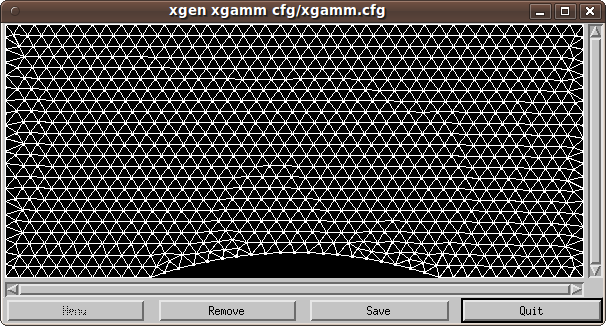
\includegraphics[width=0.8\textwidth]{xgen-2.png}
\end{center}
    \vspace{20mm}

    Version 6.0\\
    \copyright 2010 $hp$-FEM group, University of Nevada, Reno\\
    Email: hpfem-group@googlegroups.com. Home page: http://hpfem.org.

  \end{center}
  \end{titlepage}

  \section{Introduction}

  XGEN makes it possible to generate unstructured
  triangular grids on arbitrary polygonal domains. The user enters 
  a positively (= counter clock-wise) oriented boundary. Holes must 
  be oriented clock-wise. XGEN then calculates the area of the domain, and 
  throws inside an appropriate number of random points (Fig. \ref{fig:random}).

  \begin{figure}[!ht]
  \begin{center}
  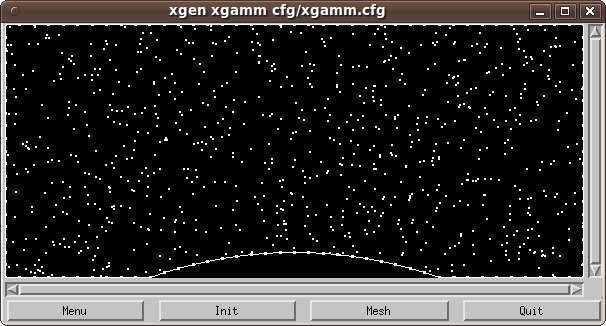
\includegraphics[width=0.8\textwidth]{xgen-4.png}
  \end{center}
  \vspace{-6mm}
  \caption{Random points.}
  \label{fig:random}
  \end{figure}
\noindent
These points are then relaxed using an ``electrostatic'' simulation
until an equilibrium is reached  (Fig. \ref{fig:equil}).

  \begin{figure}[!ht]
  \begin{center}
  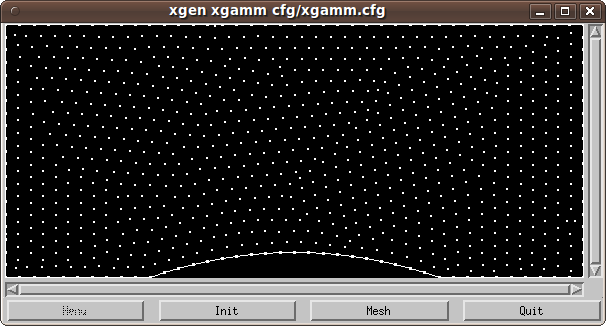
\includegraphics[width=0.8\textwidth]{xgen-5.png}
  \end{center}
  \vspace{-6mm}
  \caption{An ``electrostatic'' simulation is run to reach a local equilibrium.}
  \label{fig:equil}
\vspace{-1cm}
  \end{figure}

\newpage
\noindent
Alternativel;y, the user can choose a regular overlay pattern (Fig. \ref{fig:overlay}). 

  \begin{figure}[!ht]
  \begin{center}
  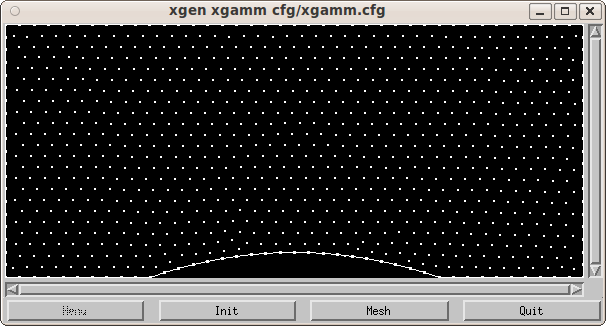
\includegraphics[width=0.8\textwidth]{xgen-1.png}
  \end{center}
  \vspace{-6mm}
  \caption{Overlay points obtained via Init $\rightarrow$ Overlay.}
  \label{fig:overlay}
  \end{figure}
\noindent 
  The user can add and remove points using the left and right mouse click,
  respectively. Mesh can be generated at any time by pressing the Mesh button.
  The Menu button launches a menu with several self-explanatory functions
  (Fig. \ref{fig:menu}). 

  \begin{figure}[!ht]
  \begin{center}
  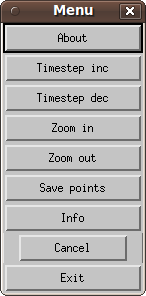
\includegraphics[width=0.2\textwidth]{xgen-3.png}
  \end{center}
  \vspace{-6mm}
  \caption{XGEN menu.}
  \label{fig:menu}
  \end{figure}
\noindent 


  \section{Compiling XGEN} \label{getting}
  
  To compile XGEN, a few libraries are needed. In Ubuntu, install them using:

{\footnotesize
\begin{verbatim}
  sudo apt-get install libmotif-dev libmotif3 lesstif2 x11proto-print-dev
\end{verbatim}
}
\noindent
  Then build XGEN by typing ``make''. The present Makefile works for
  Ubuntu Linux, but it should work on other Linux and Unix platforms with 
  no or minor modifications.
  
  \section{Creating a New Project} \label{new-project}

  To create a new project, the user has to write 
  a few lines of a simple C++ code that define a new descendant of
  a basic class Xgen. For example, let us create a class ``xsquare''
  that will triangulate a square domain. Each edge of the square 
  will be subdivided into 'N' equally long abscissas. To do this,
  one needs to add the following code to the file src/xmain.cpp.
  It was our design decision to have all projects in one file, and
  the user can change this in any way he likes.

  \begin{verbatim}
class xsquare: public Xgen {
  public:
  xsquare(char *cfg_filename) : Xgen() {XgInit(cfg_filename);}
  virtual void XgReadData(FILE *f);
};

void xsquare::XgReadData(FILE *f) {
  int N; 
  if(!Get(f, &N)) XgError("Couldn't read N.");
  XgAddEdge(3, 0, 0, N);
  XgAddEdge(2, 1, 0, N);
  XgAddEdge(4, 1, 1, N);
  XgAddEdge(1, 0, 1, N);
}
  \end{verbatim}
This tells XGEN to create a unit square domain with four edges. The first 
  edge with boundary marker '3' starts at [0, 0] and it is subdivided 
  equidistantly into 'N' intervals. An edge ends where the next one  
  starts and the end of the last edge is the starting point of the first one.
  Later we will learn how to create loops (holes) in the domain.\\
 
  \noindent
  Then add the following three lines into the main() function of the 
  file src/xmain.cpp, to make sure that the command-line parameter
  "xsquare" is recognized by XGEN and associated with the class of
  the same name:
  \begin{verbatim}
  if(!strcmp(argv[1], "xsquare")) {
    xsquare X(argv[2]);
    XgMainLoop(&X, argc, argv);
  }
  \end{verbatim}
  That's it! Create in the directory cfg/ a file that contains a single 
  integer number 'N', such as 
  \begin{verbatim}  
# This is an XGEN cfg file to project 'xsquare'.
# Number of abscissas on each edge of the square:
15
  \end{verbatim}
  Say that the name of this file is "xsquare.cfg". XGEN is run via
  \begin{verbatim}
  xgen xsquare cfg/xsquare.cfg
  \end{verbatim}
  \noindent
  The user can use additional Motif options such as:

  \begin{verbatim}  
  xgen xsquare cfg/xsquare.cfg -bg lightgray -fg blue 
  \end{verbatim}
  See the Motif1.2 Reference Guide for a list of all possible options.\\

  \noindent
  A graphical window should be launched. The user can add and remove points using 
  the left and right mouse buttons, respectively. The roles of 
  the buttons are self-explanatory. 

  \section{Mesh Output Format} \label{out_form}

  XGEN writes meshes in Hermes2D native format (http://hpfem.org/hermes).
  To override it, redefine the virtual method XgUserOutput().

  \newpage
  \noindent
  Example: 

  \begin{verbatim}
# This is an XGEN cfg file to project 'xsquare'.
# Number of abscissas on each edge of the square:
2  
  \end{verbatim}
  Now each side of the square is halved. XGEN inserts one additional point into the domain 
  that moves towards the middle. The resulting mesh has eight elements and the mesh
  file is:
  \begin{verbatim}
# XGEN mesh in Hermes2D format
# Project: xsquare
# Edges are positively oriented

# Vertices:
vertices = 
{
  { 0, 0 },
  { 0.5, 0 },
  { 1, 0 },
  { 1, 0.5 },
  { 1, 1 },
  { 0.5, 1 },
  { 0, 1 },
  { 0, 0.5 },
  { 0.499998, 0.499998 }
}

# Elements:
# (three vertex indices and a '0' (dummy material marker))
elements =
{
  { 7, 0, 8, 0 },
  { 8, 0, 1, 0 },
  { 8, 1, 3, 0 },
  { 3, 1, 2, 0 },
  { 8, 3, 5, 0 },
  { 5, 3, 4, 0 },
  { 8, 5, 7, 0 },
  { 7, 5, 6, 0 }
}

# Boundary data:
# (bdy_vrt_1 bdy_vrt_2 edge_index)
boundaries =
{
  { 0, 1, 3 },
  { 1, 2, 3 },
  { 2, 3, 2 },
  { 3, 4, 2 },
  { 4, 5, 4 },
  { 5, 6, 4 },
  { 6, 7, 1 },
  { 7, 0, 1 }
}
  \end{verbatim}

  \section{Saving and Loading Points}

  Sometimes the user may need to conserve grid point coordinates for
  further use. In ``menu'', the user can use the button ``save points''.
  To load points, use buttons ``init'' and ``load''.
  \indent
  The output file only contains points coordinates, i.e. two
  doubles per line. Reading of points finishes when end of file
  or an error while reading. Points that are checked to be
  out of the domain are ignored. This way, if the user prepares a 
  special point file with ordered points, it may take less
  time to the generator to get near the minimal potential.  

  \section{XGEN Configuration File}
   
  After calling XGEN, the generator tries to open file
  .XgenConfig in the current directory. If it is succesful,
  it tries to read as much information as possible in the
  following format:

  \begin{verbatim} 
# Path to directory with point sets:
points/
# Path to directory with meshes:
meshes/
# SubLoopsNumber:
100
# Initial size limit:
600
# Boundary redraw interval:
200
# Time step change ratio:
0.75
# Zoom ratio:
0.95
  \end{verbatim}
  Variables that are not read remain set to implicitly defined
  values. Point and grid file paths say, where the point and grid 
  files are to be stored, respectively. SubLoopsNumber is the number of
  points to be moved before returning control to the Window Manager.
  The next value is the size of the window when placed onto the screen.
  The user may notice that its shape is determined according to the shape
  of the triangulated domain by the generator itself. BoundaryRedrawInterval
  is the number of points to be moved before the boundary will be
  redrawn. TimestepConst is a number between 0 and 1 expressing the change of
  the time-step after pressing ``timestep inc'' and ``timestep dec'' in ``menu''.
  The same meaning has the last value of the file in the sense of
  zooming the domain.

  \section{Visualizing Meshes with Hermes2D}

  The easiest way to visualize an XGEN mesh is to copy the mesh file into 
  the directory ".../hermes/hermes2d/tutorial/01-mesh" in the Hermes repository, 
  comment-out local refinements
  in the main.cpp file, build the example again typing "make" in its directory, and 
  run "mesh". Then click into the graphics window containing the mesh, and press 's'
  -- this will save a BMP image on the disk. An example for the above GAMM channel
  project is shown in Fig. \ref{fig:hermes}.

  \begin{figure}[!ht]
  \begin{center}
  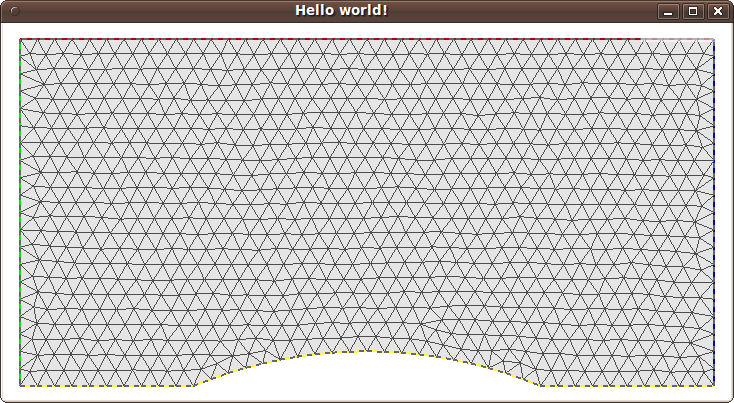
\includegraphics[width=0.8\textwidth]{xgen-6.png}
  \end{center}
  \vspace{-6mm}
  \caption{XGEN mesh visualized in Hermes2D.}
  \label{fig:hermes}
  \end{figure}


  \section{Creating User Applications} \label{vl_apl}

  The class Xgen knows all algorithms that are
  necessary to create meshes, but it is lacking a concrete geometry. 
  In order to read in a geometry, the user has to redefine the virtual 
  method

  \begin{verbatim}
    virtual void XgReadData(FILE *f) = 0;
  \end{verbatim}

  \noindent
  In addition, the user can (but does not have to) also redefine the methods
  \begin{verbatim}
    virtual double XgCriterion(Point a, Point b, Point c);
    virtual void XgUserOutput(FILE *f);
  \end{verbatim}
  In Section \ref{getting} we saw how to do this for the ``xsquare'' project.

  \section{Redefining the method XgReadData()}

  First let us look at a basic structure ``Point'' that is used by XGEN:
  \begin{verbatim}
  struct Point {
  double x, y;

  Point() {}
  Point(double ix, double iy): x(ix), y(iy) {}
  double abs() {return sqrt(x*x + y*y);}

  Point &operator += (Point B) {x += B.x; y += B.y; return *this;}
  Point &operator -= (Point B) {x -= B.x; y -= B.y; return *this;}
  Point &operator *= (double k) {x *= k; y *= k; return *this;}
  Point &operator /= (double k) {x /= k; y /= k; return *this;}
  Point &operator *= (int k) {x *= k; y *= k; return *this;}
  Point &operator /= (int k) {x /= k; y /= k; return *this;}
  Point operator + (Point B) {return Point(x + B.x, y + B.y);}
  Point operator - (Point B) {return Point(x - B.x, y - B.y);}
  Point operator * (double k) {return Point(k*x, k*y);}
  Point operator / (double k) {return Point(x/k, y/k);}
  Point operator * (int k) {return Point(k*x, k*y);}
  Point operator / (int k) {return Point(x/k, y/k);}
  double operator * (Point B) {return x*B.x + y*B.y;}
};
  \end{verbatim}  
  The method XgReadData() is given pointer to the descendant's configuration
  file (e.g. to ``xsquare.cfg'') which has been open for binary reading. The pointer
  is NULL if the file culd not be opened. User-defined XgReadData() must read from this
  file all parameters characterizing the domain in order to fill the descendant's 
  data. Shape of the domain is passed into the descendant by means of the following
  overloaded method:
  \begin{verbatim}
    void XgAddEdge(int index, double x, double y);
    void XgAddEdge(int index, Point P);
    void XgAddEdge(int index, double x, double y, int lines);
    void XgAddEdge(int index, Point P, int lines);
  \end{verbatim}
  This method adds one edge to the Xgen data structure representing the
  boundary of the triangulated domain. The boundary must be positively
  oriented. The value ``index'' means the user-defined kind of the
  corresponding boundary part (see the output format in \ref{out_form}).
  The coordinates ``x, y'' or the point ``P'' is the starting point of the edge.
  The number ``lines'' means the number of boundary edges the edge will be
  equidistantly divided into. The end point of the edge is determined either
  by adding another edge (then it is its starting point) or by calling 
  \begin{verbatim}
    void XgNewComponent();
  \end{verbatim}
  which closes the loop. Last given loop is closed automatically. 

  \section{Additional examples}

  The executable file ``xgen'' (see its source in src/xmain.cpp) contains
  some more example descendants -- there are ``xcirc'', ``xhole'', ``xgamm'', 
  ``xstep'' and ``xlist''. Run them as:
  \begin{verbatim}
    xmain xsquare cfg/xsquare.cfg &
    xmain xhole cfg/xhole.cfg &
    xmain xcirc cfg/xcirc.cfg &
    xmain xhump cfg/xhump.cfg &
    xmain xstep cfg/xstep.cfg &
    xmain xlist cfg/xlist.cfg &
  \end{verbatim}

  \section{Redefinition of the method XgCriterion()}

  This method is essential for the triangulation process. The algorithm solves
  the following task: let $ab$ be an oriented edge, points $c_1, c_2, \ldots, c_k$ lie on the left
  hand side of $ab$ (this can be written precisely). We want to choose a point $c_i$ from them
  so that the triangle
  $abc_i$ is ``the nicest one possible'' and none from the rest of points $c_j$, 
  $ i \not= j$, $j = 1, 2, \ldots, k$ lies inside of $abc_i$. Having two different
  triangles, by means of ``XgCriterion()'' we define, which one of them is nicer -- its XgCriterion
  is smaller. Each defined XgCriterion() must satisfy the following implication:
  XgCriterion(a, b, c) $<$ 
  XgCriterion(a, b, d) then the point $d$ lies outside of the triangle $abc$ for all $c, d$ lying
  on the left of $ab$.
  The implicit definition of XgCriterion(a, b, c) is

  \begin{verbatim}
double Xgen::XgCriterion(Point a, Point b, Point c) {
  return ((c-a)*(c-b))/((c-a).abs()*(c-b).abs());
}
  \end{verbatim}
%\hbox{} \hfill Pavel Solin, May 1995 (updated November 2010)


\end{document}









































